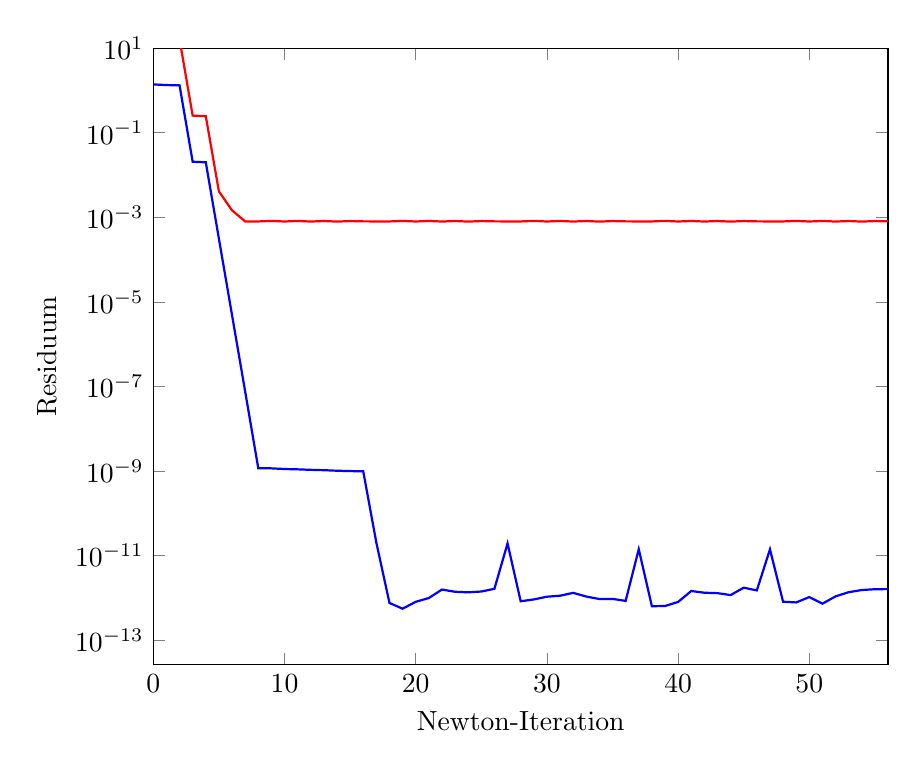
\begin{tikzpicture}[every plot/.append style={thick}] 
\begin{axis}[ 
label style={font=\normalsize}, 
xlabel={Newton-Iteration}, 
ylabel={Residuum}, 
xmin=0, xmax=56, 
ymode=log, 
ymin=0, ymax=10, 
width=0.9\textwidth, 
grid style=dashed, 
] 
\addplot[ 
color=blue, 
] 
coordinates { 
(0, 1.39e+00)(1, 1.34e+00)(2, 1.32e+00)(3, 2.06e-02)(4, 2.00e-02)(5, 3.12e-04)(6, 4.88e-06)(7, 7.63e-08)(8, 1.17e-09)(9, 1.16e-09)(10, 1.12e-09)(11, 1.10e-09)(12, 1.07e-09)(13, 1.05e-09)(14, 1.02e-09)(15, 1.00e-09)(16, 9.87e-10)(17, 2.03e-11)(18, 7.62e-13)(19, 5.57e-13)(20, 8.11e-13)(21, 9.96e-13)(22, 1.58e-12)(23, 1.40e-12)(24, 1.36e-12)(25, 1.42e-12)(26, 1.65e-12)(27, 1.95e-11)(28, 8.35e-13)(29, 9.23e-13)(30, 1.07e-12)(31, 1.13e-12)(32, 1.32e-12)(33, 1.08e-12)(34, 9.44e-13)(35, 9.50e-13)(36, 8.52e-13)(37, 1.42e-11)(38, 6.38e-13)(39, 6.45e-13)(40, 8.06e-13)(41, 1.46e-12)(42, 1.33e-12)(43, 1.30e-12)(44, 1.17e-12)(45, 1.75e-12)(46, 1.51e-12)(47, 1.41e-11)(48, 8.15e-13)(49, 7.84e-13)(50, 1.05e-12)(51, 7.32e-13)(52, 1.09e-12)(53, 1.37e-12)(54, 1.54e-12)(55, 1.61e-12)(56, 1.62e-12)}; 
\addplot[ 
color=red, 
] 
coordinates { 
(0, 1.70e+01)(1, 1.65e+01)(2, 1.62e+01)(3, 2.54e-01)(4, 2.46e-01)(5, 4.10e-03)(6, 1.46e-03)(7, 8.01e-04)(8, 8.00e-04)(9, 8.23e-04)(10, 7.97e-04)(11, 8.21e-04)(12, 7.95e-04)(13, 8.18e-04)(14, 7.93e-04)(15, 8.16e-04)(16, 8.03e-04)(17, 8.00e-04)(18, 8.00e-04)(19, 8.23e-04)(20, 7.97e-04)(21, 8.21e-04)(22, 7.95e-04)(23, 8.18e-04)(24, 7.93e-04)(25, 8.16e-04)(26, 8.03e-04)(27, 8.00e-04)(28, 8.00e-04)(29, 8.23e-04)(30, 7.97e-04)(31, 8.21e-04)(32, 7.95e-04)(33, 8.18e-04)(34, 7.93e-04)(35, 8.16e-04)(36, 8.03e-04)(37, 8.00e-04)(38, 8.00e-04)(39, 8.23e-04)(40, 7.97e-04)(41, 8.21e-04)(42, 7.95e-04)(43, 8.18e-04)(44, 7.93e-04)(45, 8.16e-04)(46, 8.03e-04)(47, 8.00e-04)(48, 8.00e-04)(49, 8.23e-04)(50, 7.97e-04)(51, 8.21e-04)(52, 7.95e-04)(53, 8.18e-04)(54, 7.93e-04)(55, 8.16e-04)(56, 8.03e-04)}; 
\end{axis} 
\end{tikzpicture} 
